% !TeX root = ../master.tex

\lecture{3}{2026-09-02}{Matrix- og Kernematerialer}

\section{Matrix- og Kernematerialer}
Matrixmaterialer er de materialer der bruges til at binde fibrene sammen med.
Typisk opdeles polymererne der bruges som matrixmateriale i hhv. hærdeplast (En: \textit{Thermosets}) og termoplast (En: \textit{Thermoplastics}).
Hærdeplast kan ikke smeltes om idet det udhærder efter første størkning, hvorimod termoplast kan smeltes om gang på gang mod en mindre forringelse af materialeevnerne.

I dette kursus vil vi hovedsageligt behandle termoplast (på trods af at industrien bruger mest hærdeplast grundet bl.a. dets bedre flyde-egenskaber), herunder bl.a.
\begin{itemize}
  \item Polyester (umættet)
  \item Vinylester
  \item Epoxy
  \item Polyurethan
  \item Cyanatester
  \item Bismaleimid
\end{itemize}
omend ikke-polymere materialer også kan bruges som matrixmateriale.

\subsection{Umættet Polyester} \label{sec:polyester}
Man kan tilføje et væld af additiver til polyester for at ændre dets egenskaber.
Monomeren i dette tilfælde er en styren, som også ses på \Mref{fig:gurit_f_13}.
Bruges mere styren fås en lavere viskositet (mere tyndtflydende) -- det er også styrenen der muliggør krydsbindingen under hærdningen.
Styren kan kendes på sin sødlige duft som vil udsive fra polyester selv mange år efter hærdning.
Der tilføres også ofte en katalysator af en art, der behjælper med at starte hærdeprocessen.
Derudover benyttes også acceleratorer, der accelererer hærdeprocessen og/eller inhibitorer der inhiberer hærdeprocessen.
Desuden kan et væld af andre additiver der bl.a. ændrer brandegenskaber, farvning, m.v. tilføjes. 

\begin{figure} [ht]
  \centering
  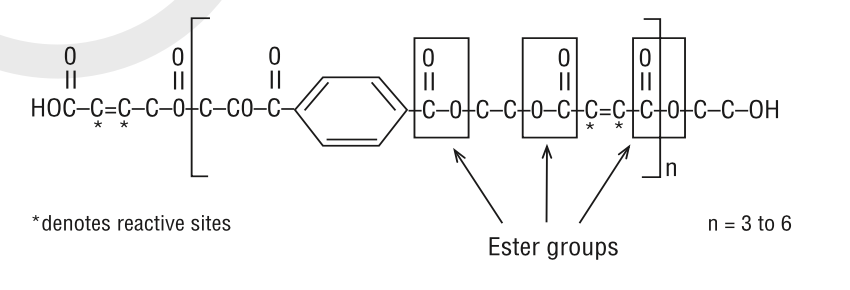
\includegraphics[width=0.8\linewidth]{./figures/gurit_f_13.png}
  \caption{Idealiseret kemisk struktur for typisk polyester, reproduceret fra \citepage{gurit2017guidecomposites}{fig. 13}.}
  \label{fig:gurit_f_13}
\end{figure}

\subsection{Vinylester} \label{sec:vinylester}
Vinylester, vist på \Mref{fig:gurit_f_16} minder på mange måder om polyester ift. mængden og typen af brugte additiver, men vinylester i sig selv har typisk bedre mekaniske egenskaber og højere kemisk bestandighed end polyesteren. 


\begin{figure} [ht]
  \centering
  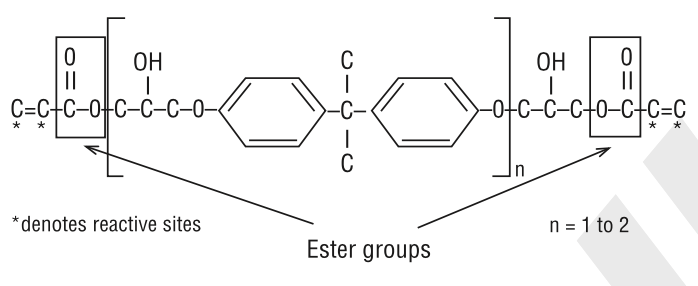
\includegraphics[width=0.8\linewidth]{./figures/gurit_f_16.png}
  \caption{Idealiseret kemisk struktur for en typisk epoxy-baseret vinylester, reproduceret fra \citepage{gurit2017guidecomposites}{fig. 16}.}
  \label{fig:gurit_f_16}
\end{figure}

\subsection{Epoxy}
Epoxy adskiller sig fundamentalt i typen af additiver fra både \Mref{sec:polyester} og \Mref{sec:vinylester}, idet det grundlæggende består af en resin som blandes med en hærder hvorefter hærdeprocessen igangsættes.
Sammenligner med de førnævnte matrixmaterialer har epoxy typisk bedre mekaniske, kemiske, elektriske og adhæssionsmæssige egenskaber. 
Dog er epoxy også mere giftigt end både \Mref{sec:polyester} og \Mref{sec:vinylester}.
\begin{figure} [ht]
  \centering
  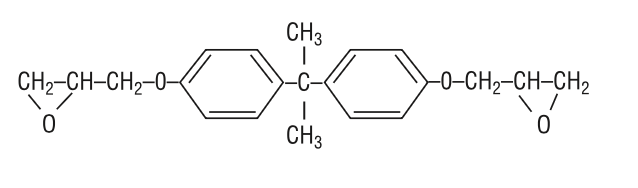
\includegraphics[width=0.8\linewidth]{./figures/gurit_f_20.png}
  \caption{Idealiseret kemisk struktur for en typisk epoxy, reproduceret fra \citepage{gurit2017guidecomposites}{fig. 20}.}
  \label{fig:gurit_f_20}
\end{figure}


\subsection{Mekaniske Egenskaber}
På \Mref{fig:gurit_f_22} ses styrken og stivheden for de tre matrix-materialer nævnt ovenfor. 
Heraf bliver det klart at epoxy generelt har bedre egenskaber end de to andre, omend de alle generelt forbedres en smule af højere temperatur.
Højere temperatur under hærdeprocessen bevirker imidlertid også at hærdeplaster ender med en højere glastransitionstemperatur. 

\begin{figure} [ht]
  \centering
  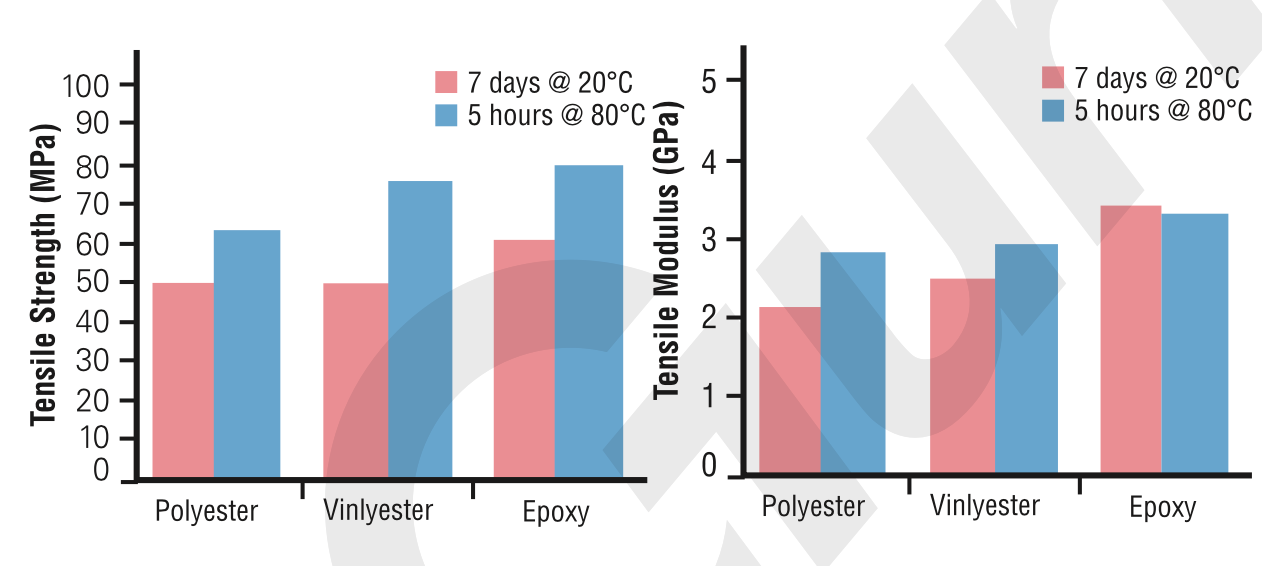
\includegraphics[width=0.8\linewidth]{./figures/gurit_f_22.png}
  \caption{Sammenligning af resinstyrke og -stivhed, reproduceret fra \citepage{gurit2017guidecomposites}{fig. 22}.}
  \label{fig:gurit_f_22}
\end{figure}

\subsection{Kernematerialer}
Kernematerialer er typisk implementeret i form af sandwich-konstruktioner, hvor et fibermateriale støbes rundt om et kernemateriale (typisk en form for meget let hårdt ``skum''), der medvirker en langt højere stivhed end en tynd fibermateriale-plade. 
